\documentclass{article}
\usepackage{amsmath}
\usepackage{booktabs}
\usepackage{caption}
\usepackage{graphicx}
\usepackage{hyperref}
\usepackage{lipsum} % For dummy text
\usepackage{subfigure} 

\begin{document}

\begin{table}[h!]
\centering
\caption{Aerosol emissions and initial conditions}
\begin{tabular*}{\linewidth}{@{\extracolsep{\fill}} cccccc}
\toprule
 Initial/Background  & $N$ (m$^{-3}$) & $D_{\text{gn}}$ ($\mu$m) & $\sigma_g$ & Composition by Mass\\
 %& 
 \midrule
Aitken Mode & $3.2 \cdot 10^9$ & 0.02 & 1.45 & 50\% (NH$_4$)$_2$SO$_4$, 50\% POA\\
Accumulation Mode & $2.9 \cdot 10^9$ & 0.116 & 1.65 & 50\% (NH$_4$)$_2$SO$_4$, 50\% POA\\
\midrule
Emissions & $E$ (m$^{-2}$ s$^{-1}$) & $D_{\text{gn}}$ ($\mu$m) & $\sigma_g$ & Composition by Mass\\
\midrule
Meat cooking & $9 \cdot 10^6$ & 0.086 & 1.9 & 100\% POA\\
Diesel vehicles & $1.6 \cdot 10^8$ & 0.05 & 1.7 & 30\% POA, 70\% BC \\
Gasoline vehicles & $5 \cdot 10^7$ & 0.05 & 1.7 & 80\% POA, 20\% BC \\
\bottomrule
\end{tabular*}
\end{table}

\begin{table}[ht]
\centering
\begin{tabular}{rrr}
  \\[-2ex]\hline 
     \hline \\[-2ex] & a & b \\ 
  \hline
1 & 1.00 & 2.00 \\ 
   \hline
2 & 1.00 & 2.00 \\ 
   \hline
\end{tabular}
\end{table}


\begin{figure}
  \centering
  \begin{subfigure}
    \centering
    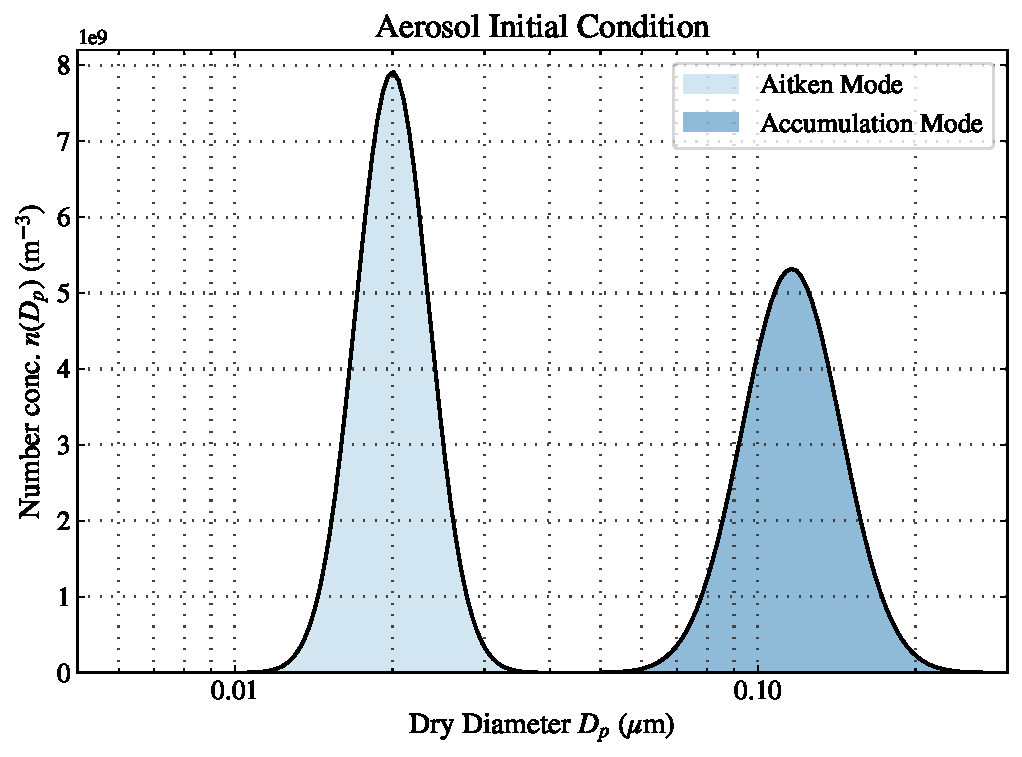
\includegraphics[width=\textwidth]{figures/urban-plume-aerosol-ic.pdf}
    \caption{Figure 1 caption}
    \label{fig:sub1}
  \end{subfigure}
   \vspace*{5mm}  % Add vertical space between figures (adjust as needed)
  \begin{subfigure}
    \centering
    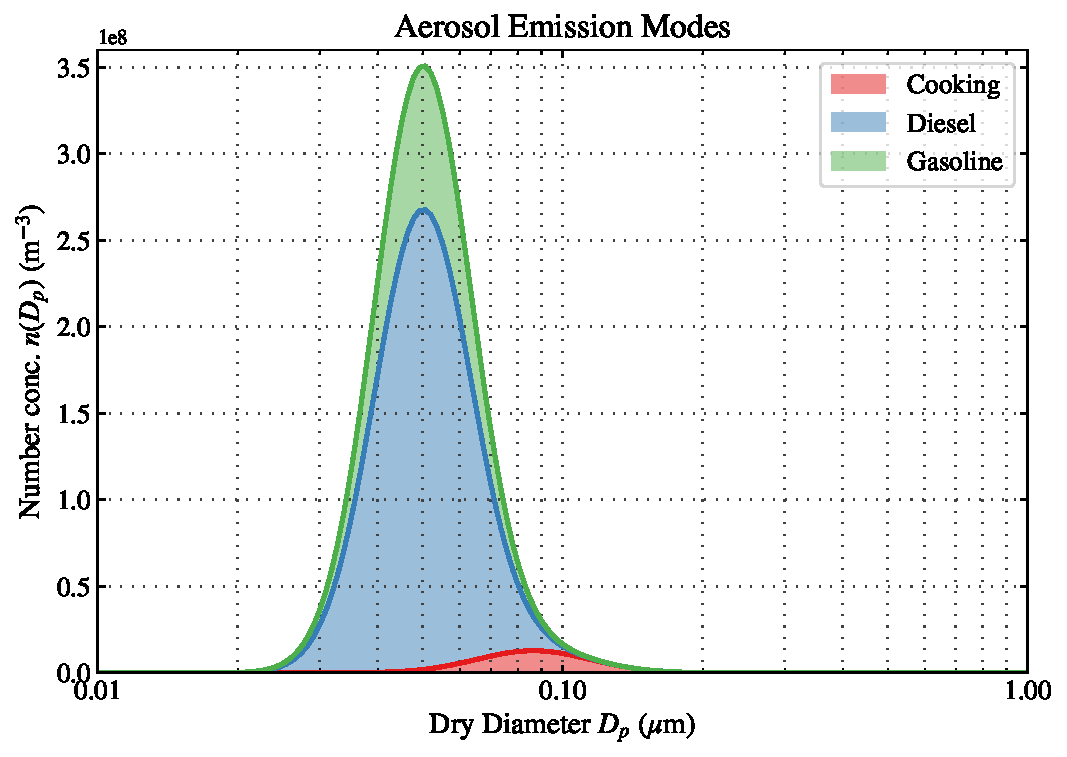
\includegraphics[width=\textwidth]{figures/urban-plume-aerosol-emissions.pdf}
    \caption{Figure 1 caption}
    \label{fig:sub1}
  \end{subfigure}
\end{figure}

\end{document}
